%%%%%%%%%%%%%%%%%%%%%%%%%%%%%%%%%%%%%%%%%%%%%%%%%%%%%%%%%%%%%%%%%%%%%%%%%%%%%% 
\newpage
\section {RMC spectrum and kMax Determination}

Measured RMC photon spectra on nuclei can be successfully described within 
the closure approximation which predicts the RMC photon spectrum depending
on just one parameter - the photon spectrum endpoint:
$$
    \frac{dN}{dE} ~=~ \frac{e^2}{\pi} \frac{k_{max}^2}{ m_{\mu}^2} (1 - \alpha) (1-x+2x^2)x(1-x)^2
$$
, where E is the photon energy, $k_{max}$ is the energy spectrum endpoint, $\rm \alpha = (N-Z)/A$,
and $x = E/k_{max}$ \cite{Christillin_1980}.

Values of $k_{max}$ for different nuclei are not predicted, but determined from the fits
to experimental data. Typically, fits return values of $k_{max}$ significantly lower that
the kinematically allowed limits. 

We determine the value of $k_{max}$ parameter by fitting the SINDRUM-II positron spectrum
with a closure approximation spectrum convoluted with the resolution $\sigma_P = 2$ MeV
and the efficiency determined from the fit to the electron spectrum
(see Figure ~\ref{fig:ana_step1_efficiency}) and varying the value of $k_{max}$.
Results of the fit are shown in Figure ~\ref{fig:ana_step2_fit_kmax}, the best fit
corresponds to $k_{max} = 88.0 \pm 0.6$ MeV.
%
With the energy losses taking into account, the value becomes  $k_{max} = 88.6 \pm 0.6$ MeV.
Maximal photon energy allowed kinematically in a 
$$
\rm \mu^- + \Au{197}(GS) \rightarrow \nu +\gamma + ^{197}Pt(GS)
$$
transition $E_{max} = 93.8$ MeV, which is several MeV higher.

\vspace{0.1in}
\begin{tikzpicture}
  \node[anchor=south west,inner sep=0] at (0,0.) {
    % \node[shift={(0 cm,0.cm)},inner sep=0,rotate={90}] at (0,0) {}
    \makebox[\textwidth][c] {
      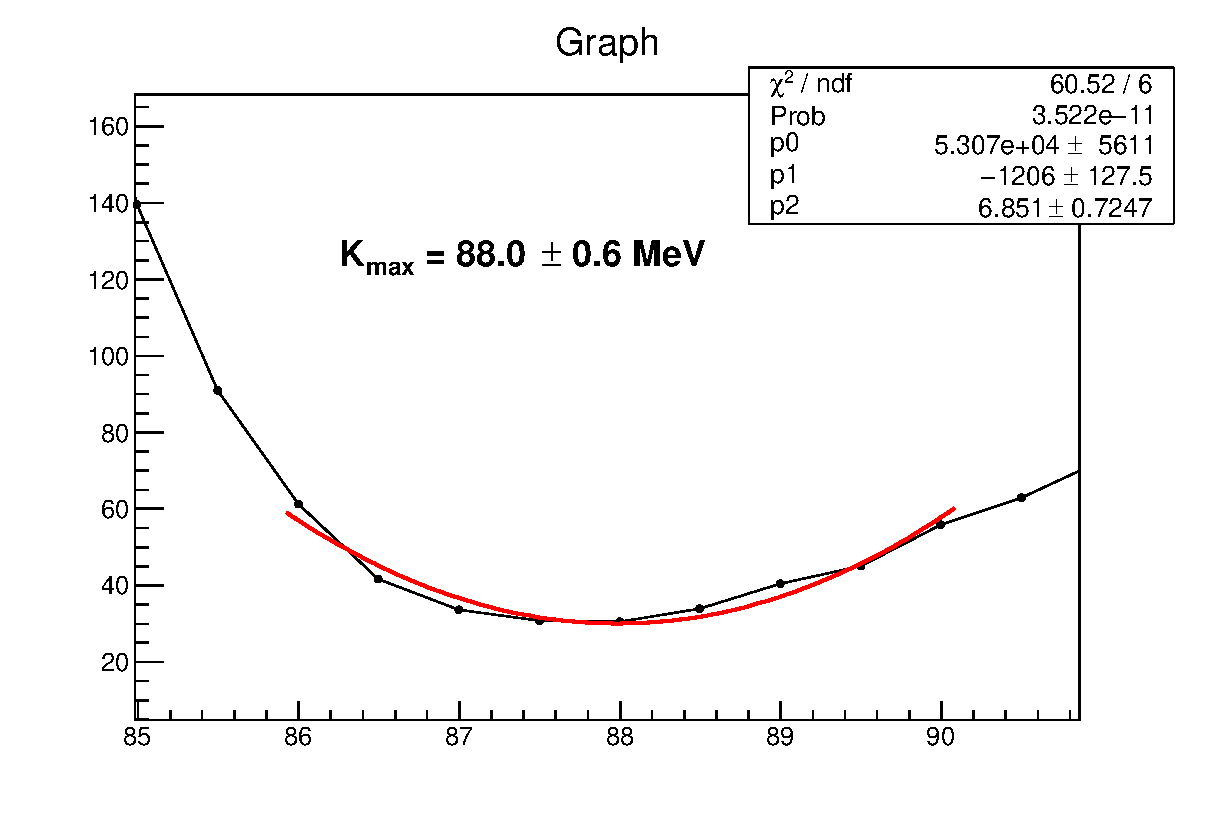
\includegraphics[width=1.0\textwidth]{figures/pdf/ana_step2_fit_kmax}
    }
  };
  % \node [text width=6cm, scale=0.8] at (4.5,6.4) {mu2e-18894 by Kevin Lynch and Jim Popp};
\end{tikzpicture}
\captionof{figure} {
  \label{fig:ana_step2_fit_kmax}
  $\chi^2$ of the SINDRUM-II positron spectrum fit with the posiron momentum distribution
  derived from the RMC closure approximation spectrum convoluted with the detector response. 
  Used in the fit are events with P < 88 MeV/c.
}
\vspace{0.1in}

%%% Local Variables:
%%% mode: latex
%%% TeX-master: t
%%% End:
